\section{Algorithmic Components}
\label{sec:algorithmic-components}

\subsection{Instrument Signature Removal}
\label{sec:acISR}
AUTHOR: Merlin
\begin{itemize}
\item Mask defects and saturation
\item Assembly
\item Overscan
\item Linearity
\item Crosstalk
\item Full frame corrections: Dark, Flats (includes fringing)
\item Pixel level corrections: Brighter fatter, static pixel size effects
\item Interpolation of defects and saturation
\item CR rejection
\item Generate snap difference
\item Snap combination
\end{itemize}

\subsubsection{AP: just skip some steps?}
AUTHOR: Simon
\begin{itemize}
\item Indicate steps to be done by camera
\item call out other steps that are omitted/modified relative to the DRP version
\end{itemize}

\subsubsection{DRP: do all the steps}
AUTHOR: Merlin


\subsection{Artifact Detection}
\label{sec:artifact}

\subsubsection{Single-Exposure Morphology}
\label{sec:acMorphologicalArtifactDetection}
AUTHOR: Simon
\begin{itemize}
\item Find CRs via morphology.
\item Find some optical ghosts (etc?) from bright star catalog and optics predictions.
\item Needs to work without PSF (amybe using placeholder PSF), but also make use of PSF if available.
\end{itemize}

\subsubsection{Single-Exposure Aggregation}
AUTHOR: Simon
\begin{itemize}
\item Find satellites via Hough transform.
\end{itemize}

\subsubsection{Snap Subtraction}
\label{sec:acSnapSubtraction}
AUTHOR: Simon
\begin{itemize}
\item All of the above, but improve by looking at both snaps.
\end{itemize}

\subsubsection{Warped Image Comparison}
\label{sec:acWarpedImageArtifactDetection}
AUTHOR: Jim
\begin{itemize}
\item Find more optical artifacts by looking at differences between warped images (this is run during background matching).
\item Find transient astronomical sources we don't want to include in coadds.
\end{itemize}

\subsection{Artifact Interpolation}
\label{sec:acArtifactInterpolation}
AUTHOR: Jim
\begin{itemize}
\item Set mask planes for all artifacts.
\item Eliminate small artifacts by interpolating them.
\item Uses PSF model as interpolant.
\end{itemize}

\subsection{Source Detection}
\label{sec:acSourceDetection}
AUTHOR: Jim
\begin{itemize}
\item Detect above-threshold regions and peaks in direct or difference images.
\item Needs to work on preconvolved and unconvolved images.
\item May need multi-pass variants: detect bright objects first, then faint; detect with approximate PSF, then improved.
\item Need to work on wavefront sensors (with out-of-focus PSFs)
\end{itemize}

\subsection{Deblending}
\label{sec:acDeblending}
AUTHOR: Jim

For templates, try:
\begin{itemize}
\item symmetry ansatz with additional regularization
\item simultaenous fit of galaxy models
\item spline-based models with regularization?
\item (multi-coadd only) optimize color uniformity
\end{itemize}

Will be especially challenging in crowded fields, but it needs to work in that regime as well.

\subsubsection{Single Frame Deblending}
\label{sec:acSingleFrameDeblending}
\begin{itemize}
\item Generate HeavyFootprint deblends using only a single image.
\item May need to be able to work with approximate/guess PSF, even in crowded fields, if we need to deblend before PSF estimation in DRP.
\item May need to work on wavefront sensors (with out-of-focus PSFs)
\end{itemize}

\subsubsection{Multi-Coadd Deblending}
\label{sec:acMultiCoaddDeblending}
\begin{itemize}
\item Generate consistent HeavyFootprint deblends from coadds over multiple bands and possibly epoch ranges.
\end{itemize}

\subsection{Measurement}
\label{sec:acMeasurement}
AUTHOR: Jim

\begin{figure}
\centering
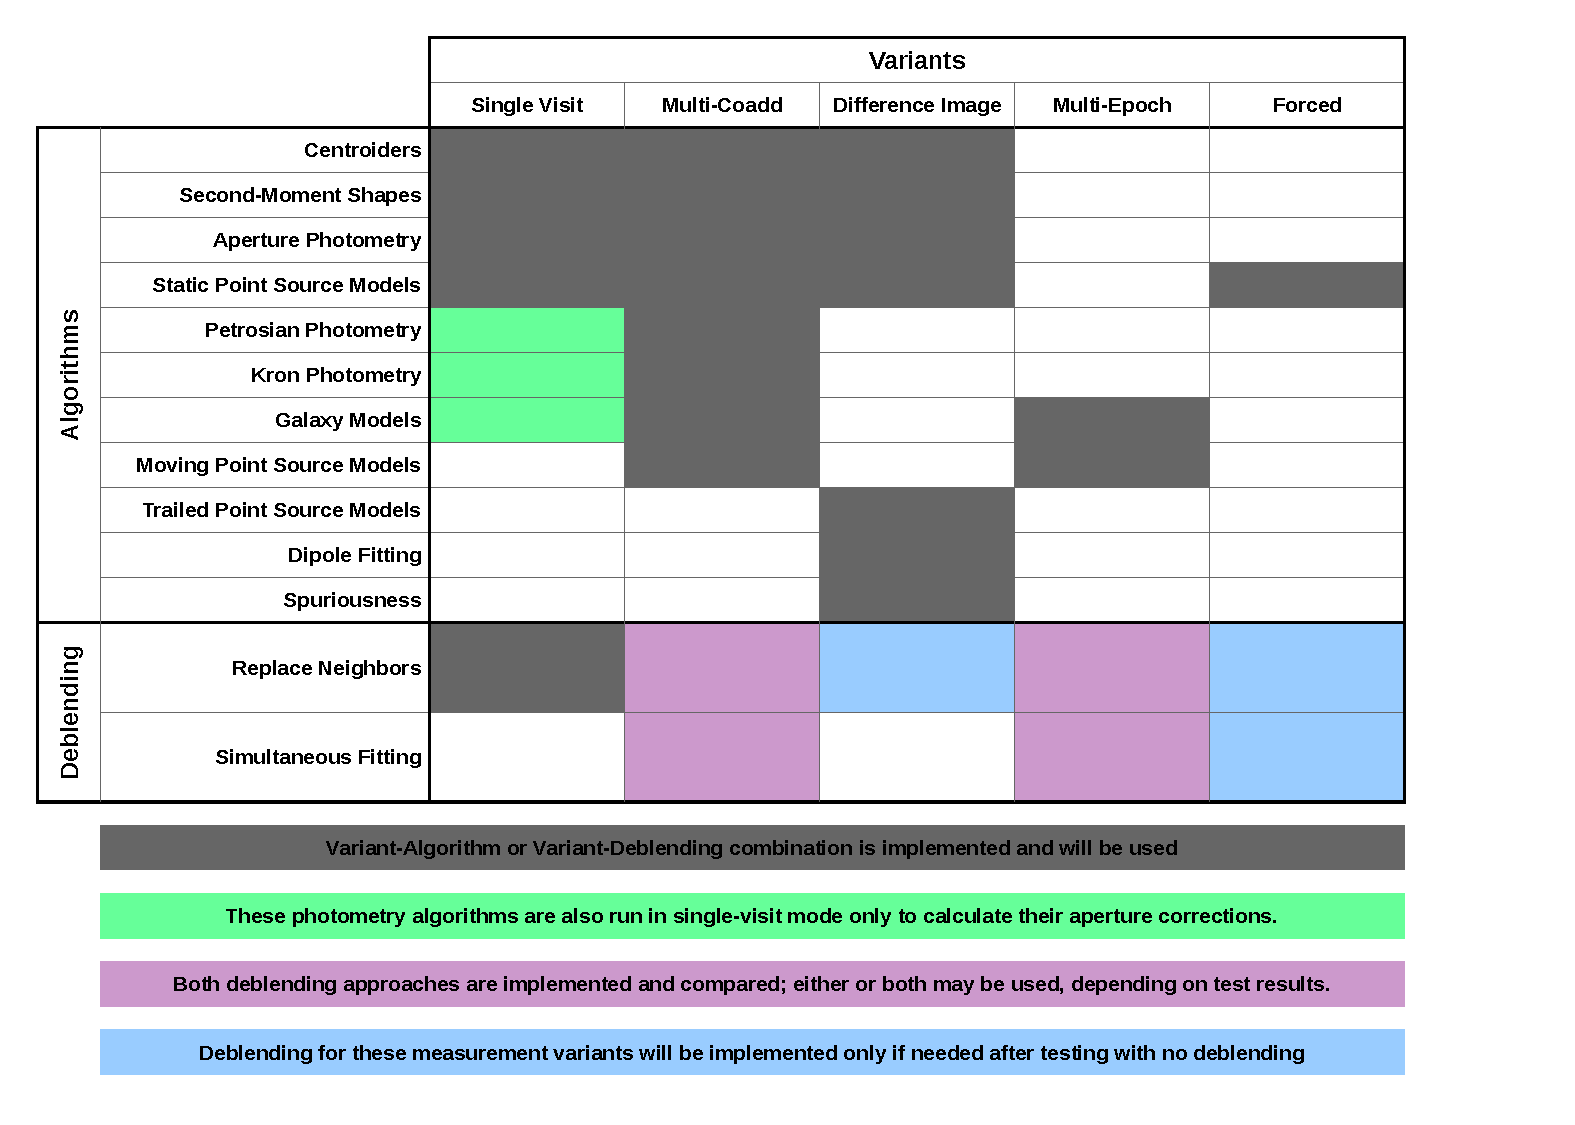
\includegraphics[width=\textwidth]{figures/measurement-matrix.pdf}
\caption{Matrix showing combinations of measurement variants, algorithms, and deblending approaches that will be implemented.
\label{fig:measurement-matrix}}
\end{figure}

\subsubsection{Variants}
Measurement is run in several contexts, but always consists of running an ordered list of algorithm plugins on either individual objects or families thereof.  Each context corresponds to different variant of the measurement driver code, and has a different set of plugin algorithms and approaches to measuring blended objects.

\paragraph{Single Frame Measurement:} Measure a direct single-visit CCD image, assuming deblend information already exists and can be used to replace neighbors with noise (see \ref{sec:acReplaceNeighborsWithNoise}).
\label{sec:acSingleFrameMeasurement}

Single Frame Measurement is run in both \hyperref[sec:apSingleFrameProcessing]{AP's Single Frame Processing pipeline}) and DRP's \hyperref[sec:drpBootstrapImChar]{BootstrapImChar}, \hyperref[sec:drpRefineImChar]{RefineImChar}, and \hyperref[sec:drpFinalImChar]{FinalImChar}.  It must be capable of running on wavefront sensor images, though this may require different plugin algorithms.

The driver for Single Frame Measurement is passed an input/output \hyperref[sec:spTablesSource]{SourceCatalog} and an \hyperref[sec:spImagesExposure]{Exposure} to measure.  Plugins take an input/output \hyperref[sec:spTablesSource]{SourceRecord} and an \hyperref[sec:spImagesExposure]{Exposure} containing only the object to be measured.

\paragraph{Multi-Coadd Measurement:} Simultaneously measure a suite of coadds representing different bandpasses, epoch ranges, and flavors.  This is run only in DRP's \hyperref[sec:drpMeasureCoadds]{MeasureCoadds} pipeline.
\label{sec:acMultiCoaddMeasurement}

The driver for Multi-Coadd Measurement is passed an input/output \hyperref[sec:spTablesObject]{ObjectCatalog} and a dict of \hyperref[sec:spImagesExposure]{Exposures} to be measured.  Plugins take an input/output \hyperref[sec:spTablesObject]{ObjectRecord} and a dict of \hyperref[sec:spImagesExposure]{Exposures}, each containing only the object to be measured.  Some plugins will also support simultanous measurement of multiple objects, which requires they be provided the subset of the \hyperref[sec:spTablesObject]{ObjectCatalog} to be measured and a dict of \hyperref[sec:spImagesExposure]{Exposures} containing just those objects.

\paragraph{Difference Image Measurement:} Measure a difference image, potentially using the associated direct image as well.  Difference image measurement is run in AP's \hyperref[sec:apAlertDetection]{Alert Detection} pipeline and DRP's \hyperref[sec:drpDiffIm]{DiffIm} pipeline.
\label{sec:acDiffImMeasurement}

The signatures of difference image measurement's drivers and algorithms are at least somewhat TBD; they will take at least a difference image \hyperref[sec:spImagesExposure]{Exposures} and a \hyperref[sec:spTablesSource]{SourceCatalog/SourceRecord}, but some plugins such as dipole measurement may require access to a direct image as well.  Because difference imaging dramatically reduces blending, difference image measurement may require any approach to blended measurement (though any use of the associated direct image would require deblending).

If preconvolution is used to construct difference images, but they are not subsequently decorrelated, the algorithms run in difference image measurement cannot be implemented in the same way as those run in other measurement variants, and algorithms that cannot be expressed as a PSF-convolved model fit (such as second-moment shapes and all aperture fluxes) either cannot be implemented or require local decorrelation.

\paragraph{Multi-Epoch Measurement:} Measure multiple direct images simultaneously by fitting the same \hyperref[sec:spWCS]{WCS}-transformed, \hyperref[sec:spPSF]{PSF}-convolved model to them.  Blended objects in Multi-Epoch Measurement will be handled by \emph{at least} fitting them simutaneously (\ref{sec:acSimultaneousFitting}), which may in turn require hybrid galaxy/star models (\ref{sec:acHybridModels}).  These models may then be used as templates for deblending and replace-with-noise (\ref{sec:acReplaceNeighborsWithNoise}) measurement if this improves the results.
\label{sec:acMultiEpochMeasurement}

Because the memory and I/O requirements for multi-epoch measurement of a single object or blend family are substantial, we will not provide a driver that accepts an \hyperref[sec:spTablesObject]{ObjectCatalog} and measures all objects within it; instead, the \hyperref{sec:drpMultiFit} pipeline will submit individual family-level jobs directly to the orchestration layer.  The multi-epoch measurement driver will thus just operate on one blend family at a time, and manage blending while executing its plugin algorithms.

Multi-epoch measurement for DRP only includes two plugin algorithms, so it is tempting to simply hard-code these into the driver itself, but this driver will also need to support new plugins in Level 3.

Multi-epoch measurement will also be responsible for actually performing forced photometry on direct images, which it can do by holding non-amplitude parameters for moving point-source models fixed and adding a new amplitude parameter for each observation.

\paragraph{Forced Measurement:} Measure photometry on an image using positions and shapes from an existing catalog.
\label{sec:acForcedMeasurement}

In the baseline plan, we assume that forced measurement will only be run on difference images; while forced photometry on direct images will also be performed in DRP, this will be done by multi-epoch measurement.

Because difference imaging reducing blending substantially, forced measurement may not require any special handling of blends.  If it does, simultaneous fitting (with point-source models) should be sufficient.

The driver for Forced Measurement is passed an input/output \hyperref[sec:spTablesSource]{SourceCatalog}, an additional input \hyperref[sec:spTablesReference]{ReferenceCatalog}, and an \hyperref[sec:spImagesExposure]{Exposure} to measure.  Plugins take an input/output \hyperref[sec:spTablesSource]{SourceRecord}, an input \hyperref[sec:spTablesReference]{ReferenceRecord} and an \hyperref[sec:spImagesExposure]{Exposure}.  If simultaneous fitting is needed to measure blends, plugins will instead receive subsets of the catalogs passed to the driver instead of individual records.

Forced measurement is used by the DRP \hyperref[sec:drpForcedPhotometry]{ForcedPhotometry} pipeline and numerous pipelines in AP.

\begin{note}[TODO]
Add references to specific AP pipelines that will use forced measurement.
\end{note}

\subsubsection{Algorithms}

\paragraph{Centroids}
\label{sec:acCentroidAlgorithms}
\begin{itemize}
\item should be equivalent to PSF model fit for stars
\item use larger weight function (TBD) for extended objects
\item need variant that doesn't require a PSF model (or can work with a poor guess) to run before PSF estimation.
\item need to have a version (possibly the main version) that works on wavefront sensors
\end{itemize}

\paragraph{Pixel Flag Aggregation}
\label{sec:acPixelFlags}
\begin{itemize}
\item Compute summary statistics of masked pixels in the neighborhood of the source/object.
\end{itemize}

\paragraph{Second-Moment Shapes}
\label{sec:acShapeAlgorithms}
\begin{itemize}
\item probably adaptive elliptical Gaussian weights, with fall back to unweightd, PSF-weighted, or some fixed Gaussian
\item add regularization for unresolved objects - avoid crazy ellipticities for objects much smaller than PSF
\item Should also compute moments of PSF model.
\item Need to have a version (possibly the main version) that works on wavefront sensors to characterize the donut-like out-of-focus sources.
\end{itemize}

\paragraph{Aperture Photometry}
\label{sec:acAperturePhotometry}

\begin{itemize}
\item Aperture fluxes are computed by summing the total flux within an elliptical region defined on the image.
\item Aperture fluxes are computed at a series of logarithmically spaced aperture sizes. Per the \DPDD{}, the total number of apertures will vary depending on the size of the source.
\item When computing fluxes for small apertures---for configurable values of ``small''--we use $\mathrm{sinc}$ interpolation \cite{Bickerton13}. For large apertures, we use a naive summation of pixel values.
\item May need to change ellipticity as a function of aperture radius.
\item If run before PSF estimation, will need a variant that does not rely on the PSF model to choose aperture size/ellipticity.
\end{itemize}

\paragraph{Static Point Source Models}
\label{sec:acStaticPointSourceModels}
\begin{itemize}
\item Fit PSF model for flux only (hold center fixed at centroid or reference value)
\item Doesn't use per-pixel variances for flux measurement, but might also provide measurement with per-pixel variances (for diagnostics?)
\end{itemize}

\paragraph{Kron Photometry}
\label{sec:acKronPhotometry}
\begin{itemize}
\item Compute Kron radius (hard to make this robust)
\item Compute flux in elliptical aperture at Kron radius.
\end{itemize}

\paragraph{Petrosian Photometry}
\label{sec:acPetrosianPhotometry}
\begin{itemize}
\item Compute Petrosian radius.  Harder than it seems due to need for improvements to splines? (ask RHL)
\item Compute flux in elliptical aperture at Petrosian radius.
\end{itemize}

\paragraph{Galaxy Models}
\label{sec:acGalaxyModels}
\begin{itemize}
\item Some sort of bulge+disk model.  Lots of need for experimentation.
\item Will Monte Carlo sample in MultiFit (and maybe on coadds, too, if that helps).
\item May also fit to PSF-matched coadds for consistent colors.
\item Will need to support simultaneous fitting (and sampling).
\item Hybrid model candidate
\end{itemize}

\paragraph{Moving Point Source Models}
\label{sec:acMovingPointSourceModels}
\begin{itemize}
\item Fit point source with flux, centroid, parallax, and proper motion parameters.
\item May need to support simultaneous fitting.
\item Might want to sample this too, at least if we fit it simultaneously with sampled galaxy models.
\item Hybrid model candidate
\end{itemize}

\paragraph{Trailed Point Source Models}
\label{sec:acTrailedPointSourceModels}
\begin{itemize}
\item Fit PSF convolved with line segment to individual images
\end{itemize}

\paragraph{Dipole Models}
\label{sec:acDipoleModels}
\begin{itemize}
\item Fit PSF dipole for separation and flux to a combination of difference image and direct image.
\item Deblending on direct image very problematic.
\end{itemize}

\paragraph{Spuriousness}
\label{sec:acSpuriousnessAlgorithms}
\begin{itemize}
\item Some per-source measure of likelhood the detection is junk (in a difference image).
\item May use machine learning on other measurements or pixels.
\item May be augmented by spuriouness measures that aren't purely per-source.
\end{itemize}

\subsubsection{Blended Measurement}
\label{sec:acBlendedMeasurement}
\begin{itemize}
\item Integrate text from blended-measurement doc here.
\end{itemize}

\paragraph{Deblend Template Projection}
\label{sec:acDeblendTemplateProjection}
\paragraph{Neighbor Noise Replacement}
\label{sec:acReplaceNeighborsWithNoise}
\paragraph{Simultaneous Fitting}
\label{sec:acSimultaneousFitting}
\paragraph{Hybrid Models}
\label{sec:acHybridModels}

\subsection{Background Estimation}
\label{sec:acBackgroundEstimation}
AUTHOR: Simon
\begin{itemize}
\item Fit or interpolate large-scale variations while masking out detections.
\item Needs to work in crowded fields.
\item Needs to work on both difference images and direct images.
\item Need to be able to compose backgrounds measured in different coordinate systems on different scales.
\item Needs to work on single CCDs for AP even if we use full FoV in DRP.
\end{itemize}

\subsection{Build Background Reference}
\label{sec:acBuildBackgroundReference}
AUTHOR: Simon
\begin{itemize}
\item Given multiple overlapping visit images (already warped to a common coordinate system), synthesize a continuous single-epoch image that can be used as a reference for background matching.
\end{itemize}

\subsection{PSF Estimation}
\label{sec:acPSFEstimation}

\subsubsection{Single CCD PSF Estimation}
\label{sec:acSingleCCDPSF}
AUTHOR: Simon
\begin{itemize}
\item Fit simple empirical PSF model to stars from a single exposure.
\item No chromaticity.
\item May use external star catalog, but doesn't rely on one.
\item Used only in Alert Production.
\end{itemize}

\subsection{Wavefront Sensor PSF Estimation}
\label{sec:acWavefrontSensorPSF}
AUTHOR: Jim
\begin{itemize}
\item Build an approximate PSF model using only the very brightest stars in the wavefront sensors.  Because WF sensors are out-of-focus, these stars may be saturated on science CCDs.
\item Model can have very few degrees of freedom (very simple optical model + elliptical Moffat/Double-Gaussian?)
\item Only needs to be good enough to bootstrap PSF model well enough to bootstrap processing of science images (but it needs to work in crowded fields, too).
\item Being able to go to brighter magnitudes may be important in crowded fields because the shape of the luminosity function may make it easier to find stars with (relatively) significant neighbors.
\end{itemize}

\subsubsection{Full Visit PSF Estimation}
\label{sec:acFullVisitPSF}
AUTHOR: Jim
\begin{itemize}
\item Decompose PSF into optical + atmosphere.
\item May also use wavefront sensors.
\item Constrain model with stars, telemetry, and wavefront data.
\item Wavelength-dependent.
\item Used in RefineImChar in DRP.
\item Must include some approach to dealing with wings of bright stars.
\end{itemize}

\subsection{Model Spatial Variation of PSF}
\subsubsection{Within a CCD}
\begin{itemize}
\item Estimate PSF at discrete locations using a set of basis functions
\item Fit interpolation functions to fit coefficients to enable interpolation
\end{itemize}
\subsubsection{Over a focal plane -- Do we need this?}

\subsection{Aperture Correction}
\label{sec:acApCorr}
AUTHOR: Jim
\begin{itemize}
\item Measure curves of growth from bright stars (visit-level, at least in DRP)
\item Correct various flux measurements to infinite (CCD-level)
\item Propagate uncertainty in aperture correction to corrected fluxes; covariance is tricky.
\end{itemize}

\subsection{Astrometric Fitting}
\label{sec:acAstrometricFitting}
AUTHOR: Simon
\subsubsection{Single CCD}
\label{sec:acSingleCCDAstrometricFit}
Used by AP, probably (RHL worries we might need full-visit)
\begin{itemize}
\item If this uses DRP's internal reference catalog, this does all we need. THIS IS A NEW DEPENDENCY BETWEEN DRP AND AP.
\end{itemize}
\subsubsection{Single Visit}
\label{sec:acSingleVisitAstrometricFit}
\begin{itemize}
\item Fit multi-component WCS to all CCDs in a single visit simultaneously after matching to reference catalog.
\end{itemize}
\subsubsection{Joint Multi-Visit}
\label{sec:acJointAstrometicFit}
\begin{itemize}
\item Fit multi-component WCS to all CCDs from multiple visits simultaneously after matching to reference catalog.
\end{itemize}

\subsection{Photometric Fitting}
\label{sec:acPhotometricFitting}
AUTHOR: Simon (and Merlin?)
\subsubsection{Single CCD (for AP)}
\label{sec:acSingleCCDPhotometricFit}
\begin{itemize}
\item Match to photometric calibration reference catalog
\item Calculate single zeropoint using available color terms
\end{itemize}
\subsubsection{Single Visit}
\label{sec:acSingleVisitPhotometricFit}
\begin{itemize}
\item Fit zeropoint (and some small spatial variation?) to all CCDs simultaneously after matching to reference catalog.
\item Need for chromatic dependence unclear; probably driven by AP.
\end{itemize}

what is this zeropoint going to be used for?  I don't see how this will add much over just the single CCD fitted zeropoints.

I think PanStarrs had a lot of success imaging a standard field every night and then just fitting a nightly zeropoint.  Twilight might be a good time to observe a standard field in all the filters that are expected to be used in the night.  Then you can have a rough zeropoint for the night and only update if conditions change?


\subsubsection{Joint Multi-Visit}
\label{sec:acJointPhotometricFit}
\begin{itemize}
\item Derive SEDs for calibration stars from colors and reference catalog classifications.
\item Utilize additional information from wavelenth dependent photometric calibration built by calibration products production.
\item Fit zeropoint and possibly perturbations to all CCDs on multiple visits simultaneously after matching to reference catalog.
\end{itemize}

My understanding for the ubercal:
\begin{itemize}
\item{you have a list of observed magnitudes that are post ISR, but pre zeropoint corrected}
\item{You can assign a rough SED to each star based on its color.}
\item{Use the atmospheric transmission information + SED of star to correct the magnitude to a fiducial filter bandpass}
\end{itemize}

Because the number of stars gets ridiculously large, I solved distinct overlapping regions of sky in parallel.  I think I used a single CCD as the patch size.  Once all the regions converge, you can run the same ubercal matrix solution to tie the patches together.  So, in equations, the fist step is to solve:
\begin{equation}
m_{ij} = m_i + z_j
\end{equation}
where $m_{ij}$ is an observed magnitude of star with true magnitude $m_i$ on observation $j$.  While it is possible to include more terms (say, fit out flat-fielding errors at the same time), that makes it much harder to solve in parallel, it's easy to make the problem degenerate, and it can slow things down rapidly. 

This method leaves a "floating zeropoint" in the solution (if you ad X to all the $m_i$'s, and -X to all the $z_j$'s the solution is the same).  If one solves regions of the sky independently, then the floating zeropoints of each region (say a HEALpixel) need to be matched:
\begin{equation}
p_{ij} = p_i + HP_j
\end{equation}
One thing that is still lacking is that it's not clear what uncertainties to put in for the different $p_{ij}$'s (unlike the observed magnitudes where it's relatively easy to calculate a reasonable uncertainty).  We also don't naturally get uncertainties out of the solvers, so that's something that needs to be worked on.

So, after solving for all the magnitudes, and merging all the patch zeropoints, there's still the final floating zeropoint (in each filter) that needs to be removed.  People like using WD for this type of thing since they have spectra that should be theoretically calculated to millimag precision.  There's also speculation that GAIA could provide a good way to do the flux calibration.  

It occurs to me that the ubercal problem can be pretty well described with a latex drawing and writing out the matrix that goes with it.  I can work on that if you want.



\subsection{Retrieve Diffim Template for a Visit}
\label{sec:acRetrieveTemplate}
AUTHOR: Simon
\begin{itemize}
\item Determine appropriate template to use
\item Generate template for observation (may include DCR correction)
\end{itemize}

\subsection{PSF Matching}
\label{sec:acPSFMatching}

The essence of image subtraction is to astrometrically register the
science image $S(x,y)$ and template image $T(x,y)$, and then match
their point spread functions (PSFs) of so that they may be subtracted
pixel by pixel. The PSFs are the time--averaged transfer functions of
a point source through the Earth's atmosphere, telescope optics, and
into the silicon of the detector before being read out. We assume that
the science image can be modeled as a convolution of the template
image by a PSF--matching kernel $\kappa(u,v;x,y)$, i.e., $S = \kappa \otimes
T$. (Indices $u,v$ indicate that the kernel itself is a 2--dimensional
function, which varies as a function of position $x,y$ in the image;
during convolution and correlation there is an implicit summation over
$u,v$.) Then the difference image, upon which new or variable sources
are detected, is given by $D = S - (\kappa \otimes T)$.

\subsubsection{Image Subtraction}
\label{sec:acImageSubtraction}
\begin{itemize}
\item Match template image to science image, as in Alert Production and DRP Difference Image processing.
\item Includes identifying sources to use to determine matching kernel, fitting the kernel, and convolving by it.
\end{itemize}

We model the PSF--matching kernel by decomposing it into a set of
basis functions $\kappa(u,v) = \sum_i a_i \kappa_i(u,v)$
\citep{Alard98}, where the coefficients are determined via
ordinary least-squares estimation:
%
\begin{eqnarray}
C_i & \equiv & (\kappa_i \otimes T); \\ \nonumber
b_{i}  & = & \sum_{x,y} {{C_i(x,y) S(x,y)}\over{\sigma^2(x,y)}};   \nonumber \\ 
M_{ij} & = & \sum_{x,y} {{C_i(x,y) C_j(x,y)}\over{\sigma^2(x,y)}};  \nonumber \\ 
a_{i}  & = & M^{-1}_{ij} b_{j}. \nonumber 
\label{eq-soln}
\end{eqnarray}
%
\noindent
$\sigma^2(x,y)$ is the per--pixel variance stored in the {\tt
  variance} plane of each LSST {\tt exposure}. To generate a spatially
varying model for the kernel, we further decompose the relative
weights of the basis coefficients $a_i$ into spatially-varying
low-order polynomials, i.e. $\kappa(u,v;x,y) = \sum_i a_i(x,y)
\kappa_i(u,v)$. We also allow for a spatially-varying differential
background between the two images $b(x,y)$ that may be fit for using a
low--order polynomial \citep{Alard98,Alard00}. The image difference is
then $D(x,y) = S(x,y) - T(x,y) \otimes \kappa(u,v;x,y) - b(x,y)$.

The basis functions $\kappa_i(u,v)$ are a degree of freedom in this
problem. Following \citep{Alard98}, we use a set of $\rm nGauss = 3$
Gaussians, each with a different width $\sigma_i$, and each modified
by a Laguerre polynomial to a given order (see below). Following more
recent studies studies \citep[e.g.][]{Israel07}, we parameterize these
different Gaussian widths via a single ratio $\beta$, such that
$\sigma_{i+1} = \beta \times \sigma_{i}$ with $\beta = 2.0$. (We note
that all constants are defined by {\tt Config} variables and may be
adjusted on a per-use basis). We set the overall scale for the
$\sigma$ by noting that, under the assumption that the PSFs of the
images are Gaussian ($\sigma_S$ for the science image and $\sigma_T$
for the template image), the $\sigma_{\kappa}$ of the matching kernel
should be simply $\sigma_{\kappa}^2 = \sigma_S^2 - \sigma_T^2$. We use
this canonical width for the central Gaussian in the basis sequences
(i.e., $\sigma_{i=2} \equiv \sigma_{\kappa}$ when using three
Gaussians bases). Each of the three default kernel basis functions are
modified by Laguerre polynomials up to order $\rm degGauss = [4, 2,
  2]$, respectively. This results in a total number of (non-spatially
varying) bases of $\sum_i^{\rm nGauss} ({\rm degGauss}_i+1)\times({\rm
  degGauss}_i+2)/2$, or 27 given the aforementioned defaults.

A spatially-invariant matching kernel $\kappa(u,v)$ is determined
separately for image substamps centered on multiple kernel candidates
across the image. The kernel candidates are selected using the {\tt
  DiaCatalogSourceSelector} to query the appropriate reference catalog
for appropriate sources to use for PSF matching. This selector allows
the user to specify the brightness and color range of the objects,
toggle star or galaxy selection, and to include variable objects or
not. Sources are vetted for signal-to-noise and masked pixels (in both
the template and science image). The matching (spatially-invariant)
kernel models $\kappa_j(u,v)$, determined for each kernel candidate $j$ as
described above, are examined and filtered by various quality
measures. The resulting ensemble of filtered kernel models is used to
constrain the spatially-varying kernel model $\kappa(u,v;x,y)$ by fitting
the spatially-varying basis kernel coefficients $a_i(x,y)$ with a
$N^{th}$-order 2-dimensional Chebyshev polynomial. This results in the
final full spatial solution $\kappa(u,v;x,y) = \sum_i a_i(x,y) \kappa_i(u,v)$,
which may be evaluated at each location $(x,y)$ in the image for
convolution.

Detection on the difference image occurs through correlation of
$D(x,y)$ with the science image's PSF, yielding optimally filtered
detection image $D'(x,y) = D(x,y) \circ PSF_S(u,v;x,y)$ where $\circ$
denotes correlation (currently the DM stack uses convolution instead
of correlation). The values of the pixels in $D'(x,y)$ provide a
maximum likelihood estimate of there being a point source at that
position. Detection occurs by simply finding pixels that are more than
$N \times \sigma$ above the square root of the per--pixel
variance. Alternatively, the science image may be {\em pre-convolved}
with a kernel similar to its PSF, in which case the resulting
difference image $D(x,y)$ is already filtered for detection. This
latter option has the additional advantage that it help us avoid
requiring {em deconvolution} of the template image, in cases when the
template has a wider PSF than the science image.

\subsubsection{PSF Homogenization for Coaddition}
\label{sec:acPSFHomogenization}
\begin{itemize}
\item Match science image to predetermined analytic PSF, as in PSF-matched coaddition.
\end{itemize}

In PSF-matched coaddition, input images are convolved by a kernel that
matches their PSF to a predefined constant PSF before they are
combined. This so-called ``model PSF matching'' uses the PSF-matching
algorithm described in the previous section to match the PSF {\em
  model} from an exposure to a pre-determined template (e.g., a
constant-across-the-sky double Gaussian) PSF model. For this task, we
realize each PSF model into an exposure-sized grid, and then utilize
those as kernel candidates as input for the PSF matching algorithm
described above.

\subsection{Image Warping}
\label{sec:acWarping}
AUTHOR: Jim
\subsubsection{Oversampled Images}
\label{sec:acOversampledWarping}

Oversampled images are warped to a new \hyperref[sec:spWCS]{WCS} and resampled using a two dimensional Lancsoz kernel of configurable order. The baselined default order is 3.

The one dimensional Lancsoz kernel of order $a$ is defined as
\[
L(x) = \begin{cases}
       \operatorname{sinc}(x)\, \operatorname{sinc}(x/a) & \text{if}\;\; -a < x < a\\ 0 & \text{otherwise.}
       \end{cases}
\]
The two dimensional Lancsoz kernel is $L(x, y) = L(x) \cdot L(y)$.

For each integer pixel position in the remapped image, the associated pixel position in the source image is determined using the source and destination WCS. The warping kernel is then applied to the source image to compute the remapped pixel value. A flux conservation factor is applied based on the relative sizes of the pixel in the source and destination WCS.

For performance reasons, it is desirable to reduce the total number of WCS calculations. It is therefore acceptable to perform the mapping between source and destination images over a regular grid and linearly interpolate between grid points, rather than mapping every pixel independently.

Since chromaticity is accounted for in the \hyperref[sec:spPSF]{PSF} rather than the WCS, no special account is taken of color when warping.

\begin{note}
The above describes the current warping implementation in afw. We should identify deficiencies with the current implementation to establish resource requirements.
\end{note}

\subsubsection{Undersampled Images}
\label{sec:acUndersampledWarping}
\begin{itemize}
\item Can use PSF model as interpolant if we also want to convolve with PSF (as in likelihood coadds).  Otherwise impossible?
\end{itemize}
\subsubsection{Irregularly-Sampled Images}
\label{sec:acFixPixelAreaVariations}
\begin{itemize}
\item Approximate procedure for fixing small-scale distortions in pixel grid.
\end{itemize}

\subsection{Image Coaddition}
\label{sec:acCoaddition}
AUTHOR: Jim
\begin{itemize}
\item Must be able to do generalized outlier rejection, using histograms of detection masks produced on difference images.
\item Needs to propagate full uncertainty somehow.
\item Needs to propagate PSFs.
\item Needs to propagate wavelength-dependent photometric calibration.
\item May need to propagate larger-scale per-exposure masks to get right PSF model or other coadded quantities.
\item Should be capable of combining coadds from different bands and/or epoch ranges ranges as well as combining individual exposures.
\item Also needs to support combining snaps
\end{itemize}

\subsection{DCR-Corrected Template Generation}
\label{sec:acDCRTemplates}
AUTHOR: Simon
\begin{itemize}
\item Somwewhat like coaddition, but may need to add dimensions for wavelength or airmass, and may involve solving an inverse problem instead of just compute means.
\end{itemize}

\subsection{Image Decorrelation}
\label{sec:acImageDecorrelation}
\subsubsection{Difference Image Decorrelation}
\label{sec:acDiffImDecorrelation}
AUTHOR: Simon
\begin{itemize}
\item Fourier-space (?) deconvolution of preconvolved difference images before measurement - ZOGY as reinterpreted by Lupton (could apply correction in real space, too)
\item Need to test with small-scale research before committing to this approach.
\end{itemize}

In situations where the signal-to-noise in the template image is not
insignificant (e.g., when the template is constructed by co-addition
of a small number of exposures), the resulting image difference will
contain autocorrelated noise arising from the convolution of the template
with the PSF matching kernel prior to subtraction. This will result in
innaccurate estimates of thresholds for {\tt diaSource} detection if
the (potentially spatially-varying) covariances in the image
difference are not properly accounted for.

A viable alternative in the case of noisy template images is to construct
an uncorrelated image by whitening the signal in the image difference
(i.e., flattening its power spectrum) \citep{Kaiser04,
 Zackay16}. This simply involves multiplying the image difference
by a term which removes its frequency dependence,

\begin{equation}
  D(k) = \left[S(k) - \kappa(k) T(k)\right]\sqrt{\frac{\sigma_S^2+\sigma_T^2}{\sigma_S^2 + \kappa^2(k)\sigma_T^2}},
  \label{eqn:decorr}
\end{equation}

\noindent
where $S$ is the science image, $T$ is the template, $\sigma_S^2$ and
$\sigma_T^2$ are their respective variances, and $\kappa$ is the
PSF-matching kernel which, when convolved with the template, matches
the PSF of the template to that of the science image. $\kappa$ may be
solved for (in real space) as described in
Section~\ref{sec:acPSFMatching}. Then the multiplication by the
square-root term in Equation~\ref{eqn:decorr} may be interpreted as
applying a post-image-differencing convolution kernel which
``removes'' the pixel-wise correlation which was added by convolution
of the template by the PSF-matching kernel. The PSF of the
resulting decorrelated difference image $\phi_D$ then equals the PSF
of the science image $\phi_S$, convolved with the post-differencing
kernel:

\begin{equation}
  \phi_D(k) = \phi_S(k) \sqrt{\frac{\sigma_S^2+\sigma_T^2}{\sigma_S^2 + \kappa^2(k)\sigma_T^2}}.
\end{equation}

We are investigating this approach and have shown that, for idealized
situations, the resulting image differences are statistically
indistinguishable from those generated using the ``Proper image
subtraction'' technique proposed by \cite{Zackay16}. 

Issues arising from complications often seen in real-world data 
such as spatially-varying PSFs and/or poorly-evaluated matching
kernels, spatially variable backgrounds and/or noise, and possibly
non-Gaussian or heteroschedastic noise need to be further
evaluated. Such tests are currently underway on simulated and real
data. These tests could highlight the advantages of the method
proposed here over the proposal of \cite{Zackay16}, including: no
requirement for accurate measurement of the science or template
images' PSFs, and thus the ability to redistribute flux in the PSF
matching to accounts for errors in astrometric alignment; and the
ability to directly account for spatially varying differential PSFs.

\subsubsection{Coadd Decorrelation}
\label{sec:acCoaddDecorrelation}
AUTHOR: Jim
\begin{itemize}
\item Fourier-space/iterative deconvolution of likelihood coadds, as in DMTN-15.
\item Need to test with small-scale research before committing to this approach.
\end{itemize}

\subsection{Star/Galaxy Classification}
\label{sec:acClassification}
AUTHOR: Jim
\subsubsection{Single Frame S/G}
\label{sec:acSingleFrameClassification}
\begin{itemize}
\item Extendedness or trace radius difference that classifies sources based on single frame measurements that can utilize the PSF model.  Used to select single-frame calibration stars, and probably aperture correction stars.
\end{itemize}
\subsubsection{Multi-Source S/G}
\label{sec:acJointCalClassification}
\begin{itemize}
\item Aggregate of single-visit S/G post-PSF numbers in jointcal.
\end{itemize}
\subsubsection{Object Classification}
\label{sec:acObjectClassification}
\begin{itemize}
\item Best classification derived from multifit and possibly variability.
\end{itemize}

\subsection{Variability Characterization}
\label{sec:acVariabilityCharacterization}

Following the \DPDD{}, lightcurve variability is characterized by providing a series of numeric summary `features' derived from the lightcurve. The DPDD baselines an approach based on Richards et al. \cite{Richards11}, with the caveat that ongoing work in time domain astronomy may change the definition, but not the number or type, of features being provided.

Richards et al. define two classes of features: those designed to characterize variability which is periodic, and those for which the period, if any, is not important. We address both below.

All of these metrics are calculated for both Objects (\DPDD{} table 4, \texttt{lcPeriodic} and \texttt{lcNonPeriodic}) and DIAObjects (\DPDD{} table 2, \texttt{lcPeriodic} and \texttt{lcNonPeriodic}). They are calculated and recorded separately in each band. Calculations for Objects are performed based on forced point source model fits (\DPDD{} table 5, \texttt{psFlux}).  Calculations for DIAObjects are performed based on point source model fits to DIASources (\DPDD{} table 1, \texttt{psFlux}). In each case, calculation requires the fluxes and errors for all of the sources in the lightcurve to be available in memory simultaneously.

\subsubsection{Characterization of periodic variability}

\begin{itemize}

\item{Characterize lightcurve as the sum of a linear term plus sinusoids at three fundamental frequencies plus four harmonics:
\begin{align}
y(t) &= ct + \sum_{i=1}^{3} \sum_{j=1}^{4} y_i(t|j f_i) \\
y_i(t|j f_i) &= a_{i,j} \sin(2 \pi j f_i t) + b_{i, j} \cos(2 \pi j f_i t) + b_{i, j, 0}
\end{align}
where $i$ sums over fundamentals and $j$ over harmonics.
}
\item{Use iterative application of the generalized Lomb-Scargle periodogram, as described in \cite{Richards11}, to establish the fundamental frequencies, $f_1$, $f_2$, $f_3$:
\begin{itemize}
  \item{Search a configurable (minimum, maximum, step) linear frequency grid with the periodogram, applying a $\log f/f_N$ penalty for frequencies above $f_N = 0.5 \langle 1 / \Delta T \rangle$, identifying the frequency $f_1$ with highest power;}
  \item{Fit and subtract that frequency and its harmonics from the lightcurve;}
  \item{Repeat the periodogram search to identify $f_2$ and $f_3$.}
\end{itemize}
}
\item{We report a total of 32 floats:
  \begin{itemize}
  \item{The linear coefficient, $c$ (1 float)}
  \item{The values of $f_1$, $f_2$, $f_3$. (3 floats)}
  \item{The amplitude, $\mathrm{A}_{i, j} = \sqrt{a_{i, j}^2 + b_{i, j}^2}$, for each $i, j$ pair. (12 floats)}
  \item{The phase, $\mathrm{PH}_{i, j} = \arctan(b_{i, j}, a_{i, j}) - \frac{j f_i}{f_1} \arctan(b_{1,1}, a_{1,1})$, for each $i, j$ pair, setting $\mathrm{PH}_{1, 1} = 0$. (12 floats)}
  \item{The significance of $f_1$ vs. the null hypothesis of white noise with no periodic signal. (1 float)}
  \item{The ratio of the significance of each of $f_2$ and $f_3$ to the significance of $f_1$. (2 floats)}
  \item{The ratio of the variance of the lightcurve before subtraction of the $f_1$ component to its variance after subtraction. (1 float)}
  \end{itemize}
NB the \DPDD{} baselines providing 32 floats, but, since $\mathrm{PH}_{1,1}$ is 0 by construction, in practice only 31 need to be stored.
}
\end{itemize}

\subsubsection{Characterization of aperiodic variability}

In addition to the periodic variability described above, we follow \cite{Richards11} in providing a series of statistics computed from the lightcurve which do not assume peridoicity. They define 20 floating point quantities in four groups which we describe here, again with the caveat that future revisions to the \DPDD{} may require changes to this list.

Basic quantities:

\begin{itemize}
\item{The maximum value of delta-magnitude over delta-time between successive points in the lightcurve.}
\item{The difference between the maximum and minimum magnitudes.}
\item{The median absolute deviation.}
\item{The fraction of measurements falling within $1/10$ amplitudes of the median.}
\item{The ``slope trend'': the fraction of increasing minus the fraction of decreasing delta-magnitude values between successive pairs of the last 30 points in the lightcurve.}
\end{itemize}

Moment calculations:

\begin{itemize}
\item{Skewness.}
\item{Small sample kurtosis, i.e.
\begin{align}
\mathrm{Kurtosis} &= \frac{n(n+1)}{(n-1)(n-2)(n-3)} \sum_{i=1}^{n} \left(\frac{x_i - \overline{x}}{s}\right)^4 -\frac{3(n-1)^2}{(n-2)(n-3)} \\
s &= \sqrt{\frac{1}{n-1} \sum_{i=1}^{n}(x_i - \overline{x})^2}
\end{align}
}
\item{Standard deviation.}
\item{The fraction of magnitudes which lie more than one standard deviation from the weighted mean.}
\item{Welch-Stetson variability index $J$ \cite{Stetson96}, defined as
\[
J = \frac{\sum_{k} \mathrm{sgn}(P_k) \sqrt{|P_k|}}{K},
\]
where the sum runs over all $K$ pairs of observations of the object, where $\mathrm{sgn}$ returns the sign of its argument, and where
\begin{align}
P_k &= \delta_i \delta_j \\
\delta_i &= \sqrt{\frac{n}{n-1}}\frac{\nu_i - \overline{\nu}}{\sigma_{\nu}},
\end{align}
where $n$ is the number of observations of the object, and $\nu_i$ its flux in observation $i$. Following the procedure described in Stetson \cite{Stetson96}, the mean is not the simple weighted algebraic mean, but is rather reweighted to account for outliers.}
\item{Welch-Stetson variability index $K$ \cite{Stetson96}, defined as
\[
K = \frac{1/n \sum_{i=1}{N}|\delta_i|}{\sqrt{1/n \sum_{i=1}{N}|\delta_i^2|}},
\]
where $N$ is the total number of observations of the object and $\delta_i$ is defined as above.}
\end{itemize}

Percentiles. Taking, for example, $F_{5,95}$ to be the difference between the $95\%$ and $5\%$ flux values, we report:

\begin{itemize}
\item{All of $F_{40,60} / F_{5,95}$, $F_{32.5,67.5} / F_{5,95}$, $F_{25,75} / F_{5,95}$, $F_{17.5,82.5} / F_{5,95}$, $F_{10,90} / F_{5,95}$}
\item{The largest absolute departure from the median flux, divided by the
median.}
\item{The radio of $F_{5,95}$ to the median.}
\end{itemize}

QSO similarity metrics, as defined by Butler \& Bloom \cite{Butler11}:

\begin{itemize}
\item{$\chi_{\mathrm{QSO}}^2 / \nu$.}
\item{$\chi_{\mathrm{False}}^2 / \nu$.}
\end{itemize}

\subsection{Proper Motion and Parallax from DIASources}
\label{sec:acStellarMotionFitting}
AUTHOR: Simon
\begin{itemize}
\item Fit proper motion and parallax models to all potisions of DIASources belonging to a DIAObject taking into account errors.
\end{itemize}

\subsection{Association and Matching}
\label{sec:acMatching}
\subsubsection{Single CCD to Reference Catalog, Semi-Blind}
\label{sec:acSingleCCDReferenceMatching}
AUTHOR: Simon
\begin{itemize}
\item Want to match in image coordinates, so also needs to transform reference catalog.
\item Run prior to single-visit WCS fitting, with only telescope's best guess as a starting WCS.
\item Single CCD form needed by AP.
\end{itemize}

\subsubsection{Single Visit to Reference Catalog, Semi-Blind}
\label{sec:acSingleVisitReferenceMatching}
AUTHOR: Simon
\begin{itemize}
\item Want to match in focal plane coordinates, so also needs to transform reference catalog.
\item Run prior to single-visit WCS fitting, with only telescope's best guess as a starting WCS.
\end{itemize}

\subsubsection{Multiple Visits to Reference Catalog}
\label{sec:acJointCalMatching}
AUTHOR: Jim
\begin{itemize}
\item Match sources from multiple visits to a single reference catalog, assuming good WCS solutions.
\end{itemize}

\subsubsection{N-Way Matching Across Multiple Visits}
\label{sec:acNWayMatching}
AUTHOR: MWV
\begin{itemize}
\item Match sources and associate objects from M catalogs each with $\sim$N sources.  The API should match in either (x, y) or (RA, Dec).  Positions for source detections solutions will be assumed to already be correct.  Order of individual catalogs should not matter.  Algorithm will need to be able to run on M$\sim$1,000 visits.  Such a tool will allow flexible analyses without the requirement for a larger database structure or full coadd-based object identifiction and forced photometry.  Even within the framework of a complete Level-2 DRP release, such a N-way matching capability will also be important for comparing the results of single-visit photometry with the deep coadd-based object detection and forced photometry.  A specific example use case for lightweight quality assessment is taking the processed catalogs for M=1,000 images each with N=2,000 sources and creating object associations add derived repeatability and time-variable summary statistics.  This algorithm and associated API should provide a general purpose tool useful for algorithm developers, data quality assessment, and science users.  A trivial in-memory version (using full catalogs), a streamlined in-memory version (load only the coordinates), and a larger-than-memory version will each be useful and important and will entail increasingly more significant design and performance efforts.
\end{itemize}

\subsubsection{DIAObject Generation}
\label{sec:acDIAObjectGeneration}
AUTHOR: Simon
\begin{itemize}
\item Match all DIASources to predicted Solar System object positions and existing DIAObjects and generate new DIAObjects.  Definitely run in AP, maybe run in DRP.
\end{itemize}

\subsubsection{Object Generation}
\label{sec:acObjectGeneration}
AUTHOR: Jim
\begin{itemize}
\item Match coadd detections from different bands/SEDs/epoch-ranges, merging Footprints and associating peaks.
\item Also merge in DIASources or (if already self-associated) DIAObjects.
\end{itemize}

\subsubsection{Blended Overlap Resolution}
\label{sec:acBlendedOverlapResolution}
AUTHOR: Jim
\begin{itemize}
\item Given two or more overlapping blend families (with associated measurements), merge them by selecting the ``best'' measurement for each child object.
\end{itemize}

\subsection{Raw Measurement Calibration}
\label{sec:acRawMeasurementCalibration}

AUTHOR: Jim
\begin{itemize}
\item Apply astrometric and photometric calibrations to measurements in raw units, transforming them to calibrated quantities.
\item May be applied within the database after ingest in some contexts, but needs to be available outside the database as well.
\end{itemize}


\subsection{Ephemeris Calculation}
\label{sec:acEphemerisCalculation}
AUTHOR: Simon
\begin{itemize}
\item Calculate positions for all solar system objects in a region at a given time.
\end{itemize}

\subsection{Make Tracklets}
\label{sec:acMakeTracklets}
AUTHOR: Simon
\begin{itemize}
\item Make all tracklet pairs
\item Merge multiple chained observation into single longer tracklets
\item Purge any tracklets inconsistent with the merged tracklets
\end{itemize}

\subsection{Attribution and precovery}
\label{sec:acAttributionAndPrecovery}
AUTHOR: Simon
\begin{itemize}
\item Predict locations of known Solar System objects
\item Match tracklet observation to predicted ephimerides taking into account velocity
\item Update SSObjects
\item Possibly iterate
\end{itemize}

\subsection{Orbit Fitting}
\label{sec:acOrbitFitting}
AUTHOR: Simon
\begin{itemize}
\item Merge unassociated tracklets into tracks.
\item Fit orbits to all tracks.
\item Purge unphysical tracks.
\item Update SSObjects
\item Possibly iterate
\end{itemize}
